
The results of this thesis are divided into three different sections. Section \ref{sec:results_anharm} focuses on the microscopic modeling of anharmonic effects in phononic thermal conduction at interfaces and in quasi-one-dimensional nanowires. Section \ref{sec:results_interference} demonstrates interference effects observed in classical phonon thermal conduction through microscopic point contacts and shows how the effects are washed away by increasing temperature. Finally, Section \ref{sec:results_gf} presents highlights from the Green's function modeling, which is applied to (i) account for quantum statistics in phonon transport through point contacts and (ii) demonstrate the cavity-enhancement of interparticle energy transfer between SiO$_2$ nanoparticles.

\section{Anharmonic effects in phononic thermal conduction}
\label{sec:results_anharm}

This Section presents non-equilibrium molecular dynamics simulation results for phononic thermal conduction with special attention to anharmonic effects. Subsection \ref{sec:results_interface} considers interfacial thermal conduction between two planar mass-mismatched lattices, summarizing the results of \citepub{spectral}. Subsection \ref{sec:results_mfps} reviews the results for frequency-dependent phonon mean free paths in carbon nanotubes, published in \citepub{cnt}. Finally, Subsection \ref{sec:results_twinning} re-caps the results of \citepub{twinning} on the thermal conductivity reduction by lattice twinning in silicon nanowires.

\subsection{Interfacial thermal conductance (\citepub{spectral})}
\label{sec:results_interface}
% \begin{figure}[tb]
%  \begin{center}
%   %\includegraphics[width=.99\columnwidth]{/Users/saaskilak/Documents/matlab/pics/171213a_cnt.ps}
%  % \includegraphics[width=.99\columnwidth]{/Users/saaskilak/Documents/latex/pics/240114_fcc_final.ps}
%   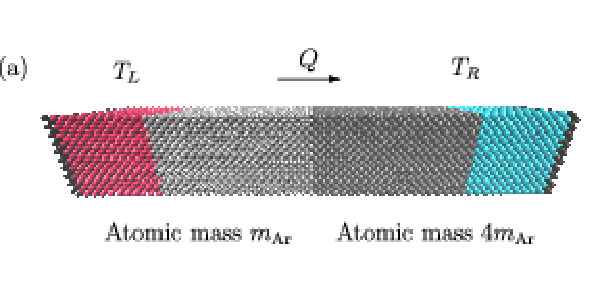
\includegraphics[width=8.6cm]{pics/nemd_fig2a.pdf}
%   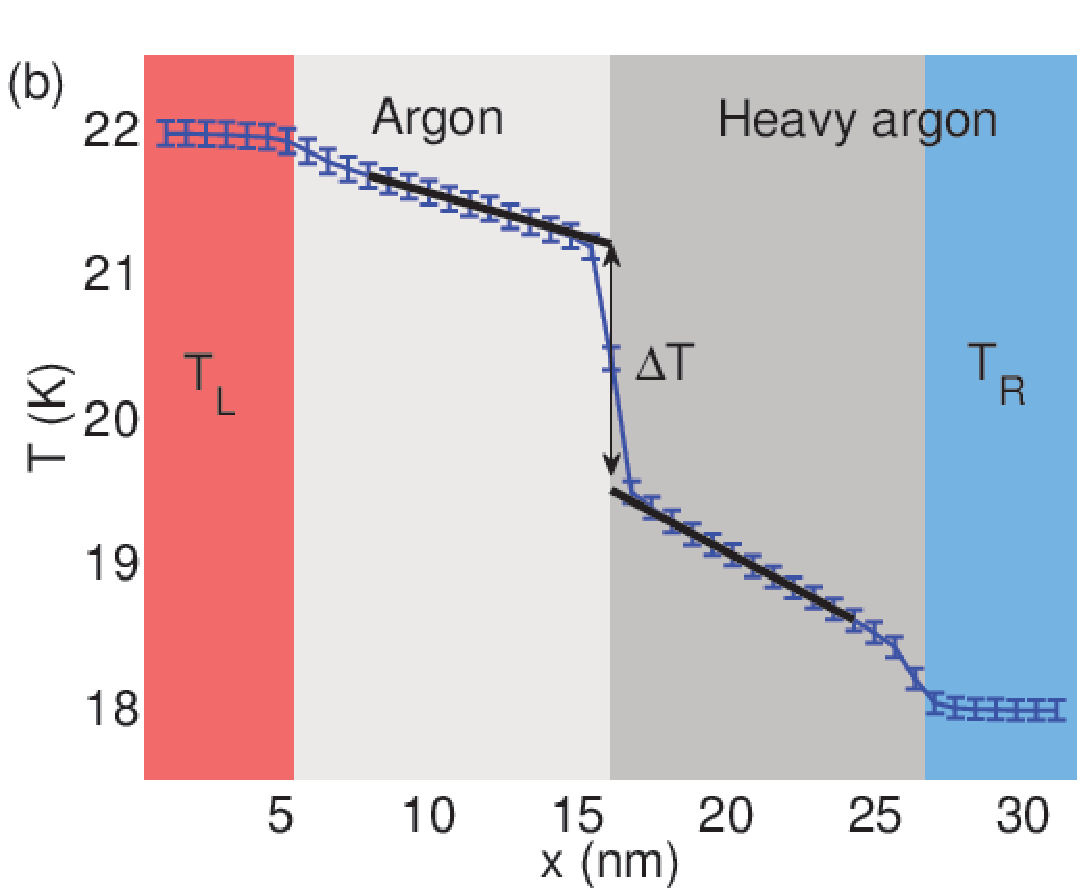
\includegraphics[width=8.6cm]{pics/nemd_fig2b.pdf}
%   \caption{(a) Atomistic illustration of the studied interface between two mass-mismatched Lennard-Jones solids. The atoms at the left and right ends are coupled to Langevin heat baths at different temperatures $T_L$ and $T_R$ to drive thermal current $Q$ through the interface in the middle. (b) Local kinetic temperature profile in a non-equilibrium simulation with average temperature $T=20$ K. Temperature drop $\Delta T$ at the interface is estimated by extrapolating the linear fits to the temperature profiles at different sides of the interface and calculating the difference at the interface. } 
%  \label{fig:nemd_fig1}
%  \end{center}
% \end{figure}

The role of anharmonic phonon scattering in interfacial thermal conduction was investigated using the computational setup presented earlier in Fig. \ref{fig:th_spectral_geom}. Two face-centered cubic lattices with similar lattice vectors were in perfect, planar contact along the [100] lattice direction. Interatomic interactions were modeled using the Lennard-Jones potential \cite{allentildesley} and the parameters were chosen to correspond to solid argon. To model acoustic mismatch between the materials, the atomic mass at one side of the interface was chosen to be four times larger than on the other side, where the atomic mass was chosen to correspond to solid argon. More simulation details are found in \citepub{spectral}.

\begin{figure}[tb]
 \begin{center}
  %\includegraphics[width=.99\columnwidth]{/Users/saaskilak/Documents/matlab/pics/171213a_cnt.ps}
 % \includegraphics[width=.99\columnwidth]{/Users/saaskilak/Documents/latex/pics/240114_fcc_final.ps}
  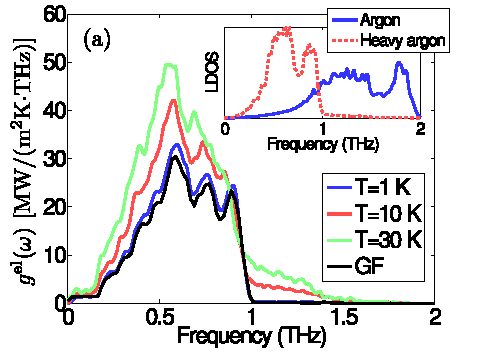
\includegraphics[width=.49\columnwidth]{pics/nemd_fig4a.pdf}
  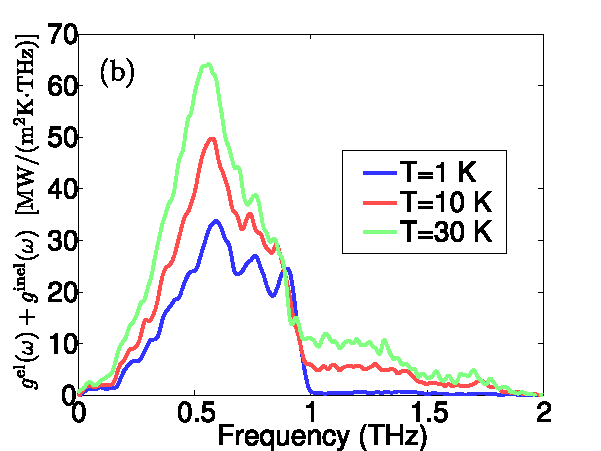
\includegraphics[width=.49\columnwidth]{pics/nemd_fig4b.pdf}
  \caption{The conductance $g^{\textrm{el}}(\omega)=q(\omega)/\Delta T_b$ as a function of frequency at various temperatures. At $T=1$ K, the elastic conductance agrees very well with the Landauer-B\"uttiker conductance calculated using the Green's function (GF) method. At high temperatures, anharmonic scattering in the bulk enables energy transfer even above the cut-off frequency of the heavier solid, located at 1 THz. Inset: Local density of vibrational states (LDOS, arbitrary units) at the interface. Although phonons cannot propagate in the heavier bulk above 1 THz, there are evanescent wave states extending up to 1.5 THz at the vicinity of the interface. (b) The sum $g^{\textrm{el}}(\omega)+ g^{\textrm{inel}}(\omega)$ of elastic and inelastic spectral conductance as a function of frequency. The inelastic conductance has been defined in detail in \citepub{spectral}. At high temperatures, the anharmonic energy transfer processes strongly enhance interfacial heat transfer at $f\approx 0.5$ THz and above the cut-off of the heavier material (1 THz). Figure reprinted with publisher's permission from \citepub{spectral}.} 
 \label{fig:nemd_fig2}
 \end{center}
\end{figure}

Interfacial heat transfer mechanisms were investigated by calculating the spectral heat current \eqref{eq:th_spectral_curr} for all atomic pairs interacting across the interface. By varying the mean temperature $T$, one can investigate the role of anharmonic effects. Figure \ref{fig:nemd_fig2}(a) shows the spectral conductance $q(\omega)/\Delta T_b$, defined as the spectral current divided by the temperature jump at the interface, for different temperatures. At the low temperature of $T=1$ K, the conductance agrees remarkably well with the harmonic Green's function calculation. At higher temperatures, the onset of anharmonic effects can be seen to assist energy transfer across the interface. Most notably, anharmonic effects enable energy transfer even above the cut-off frequency of the heavier material, located at $1$ THz. Because these high-frequency modes cannot propagate in the heavier material, they can only dissipate their heat in the immediate vicinity of the interface by anharmonic effects. Such evanescent wave dissipation has not been identified from microscopic simulations in earlier literature.

To further probe the anharmonic contributions to thermal conductance, the second-order contribution to the spectral heat current was also calculated from MD simulation. These contributions arise from three-phonon energy transfer processes directly at the interface. The sum of first- and second-order contributions to the conductance is shown in Fig. \ref{fig:nemd_fig2}(b). The three-phonon processes can be seen to enhance energy transfer across the whole frequency range between zero and 2 THz,  both below and above the cut-off frequency of the heavy argon. As discussed in detail in \citepub{spectral}, the three-phonon energy tranfer processes are dominated by frequency-doubling and frequency-halving anharmonic processes at the interface, in support of the phenomenological higher harmonic inelastic model (HHIM) suggested by Hopkins \cite{hopkins09_jap}.

\subsection{Mean free paths in carbon nanotubes (\citepub{cnt})}

\label{sec:results_mfps}

\begin{figure}[tb]
 \begin{center}
  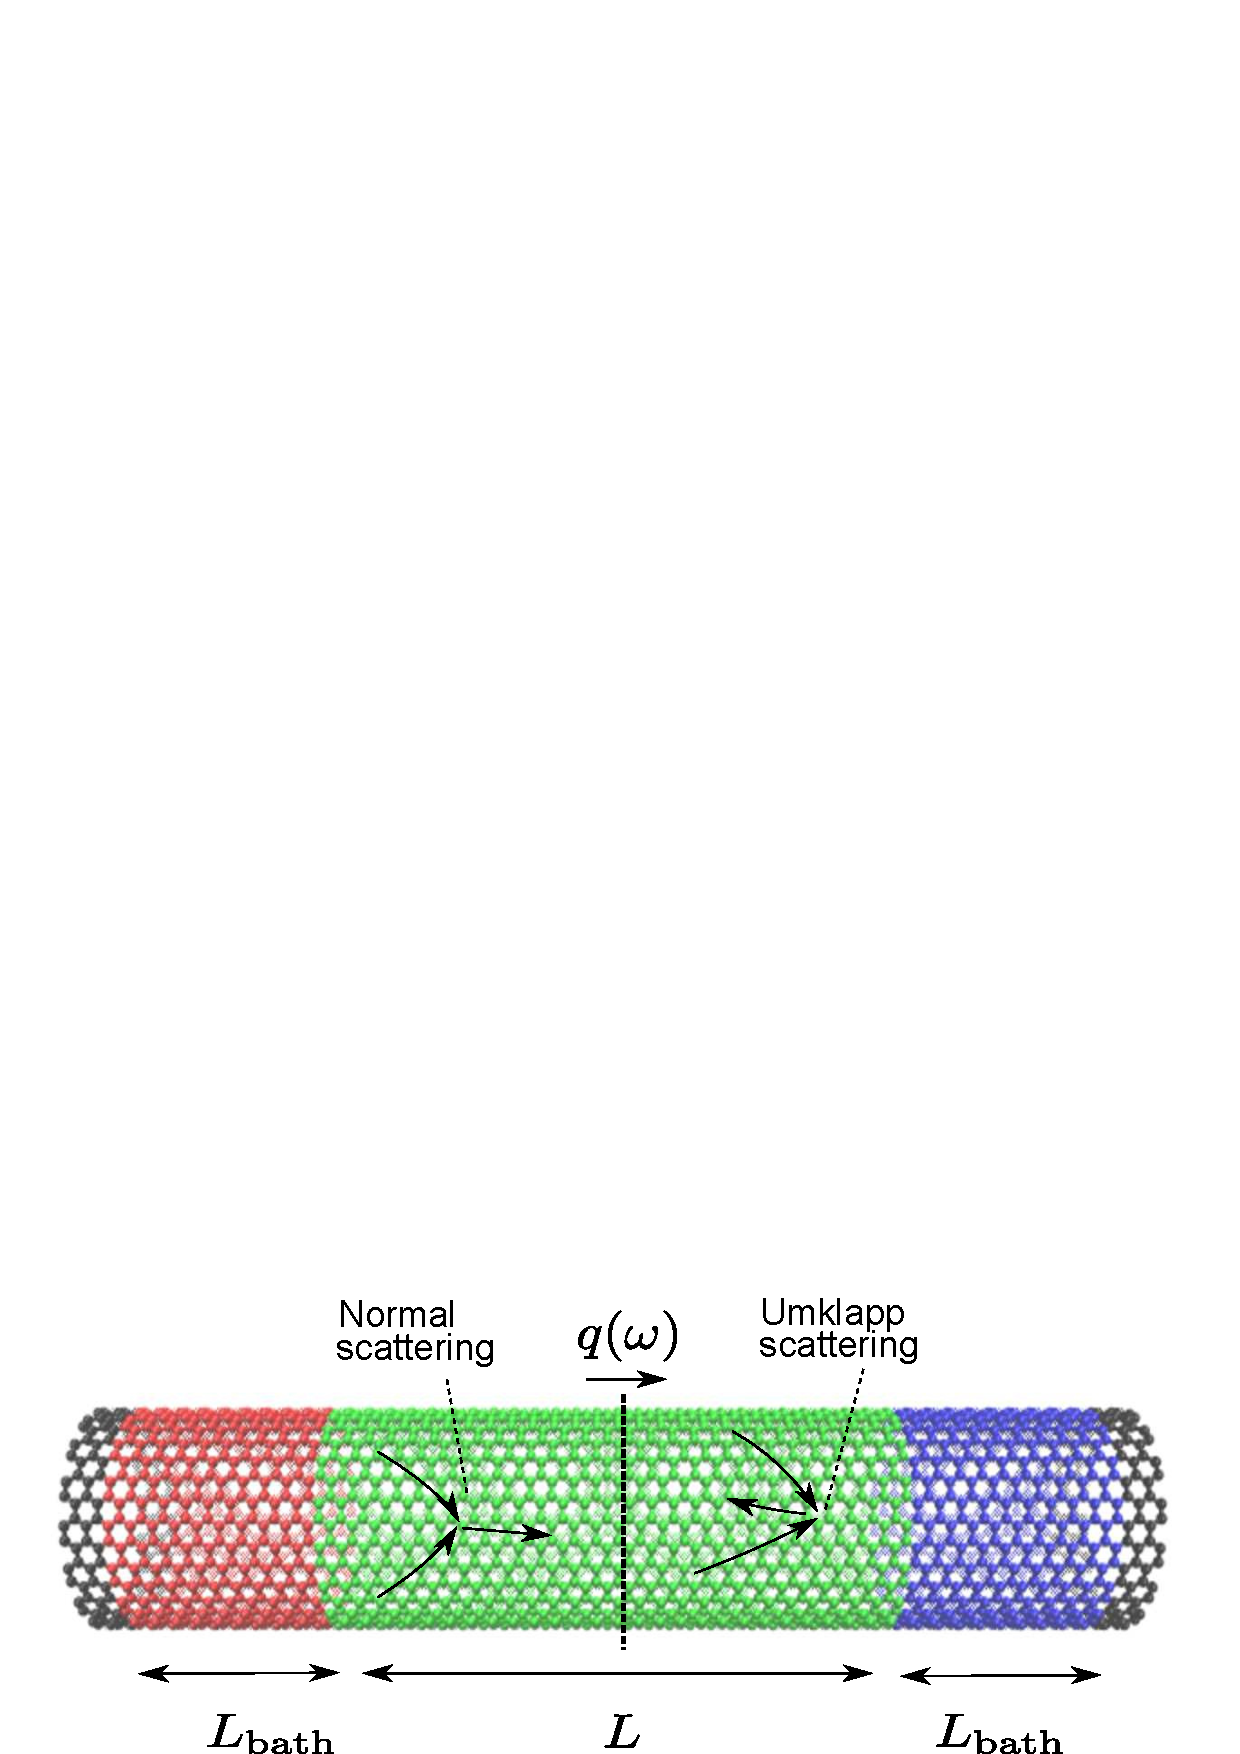
\includegraphics[width=.89\columnwidth]{pics/cnt_fig1.pdf} 
  \caption{Schematic illustration of the NEMD setup used for determining the length-dependent thermal conductivity and phonon mean free paths in carbon nanotubes. When traversing the tube, phonons undergo both normal and Umklapp processes leading to the length-dependence of the spectral heat current $q(\omega)$ in the tube. From the $L$-dependence of $q(\omega)$, one can determine the mean free paths at each frequency as described in \citepub{cnt}. Figure reprinted with publisher's permission from \citepub{cnt}.}  
\label{fig:cnt_fig1}
 \end{center}
\end{figure}

Figure \ref{fig:cnt_fig1} shows the schematic illustration of the NEMD setup used for determining phonon mean free paths in (10,10) carbon nanotubes in \citepub{cnt}. Regions of length $L_{\textrm{bath}}=10$ nm were coupled to Langevin thermostats to drive heat current through the tube, and the frequency-dependent phonon mean free paths were determined from the decrease of the non-equilibrium spectral heat current \eqref{eq:th_spectral_curr} at different frequencies as a function of tube length $L$. The decrease in spectral current arises from anharmonic interactions, which are fully accounted for by the non-linear terms of the optimized Tersoff potential used for modeling carbon-carbon interactions \cite{tersoff88a,lindsay10}. In contrast to equilibrium mean free paths, which characterize the scattering lengths for both normal and Umklapp processes \cite{mcgaughey04}, the mean free paths determined from NEMD reflect the \textit{resistance to the heat flow} (dominated by Umklapp processes). For a detailed account of the method, see \citepub{cnt}.


\begin{figure}[tb]
 \begin{center}
  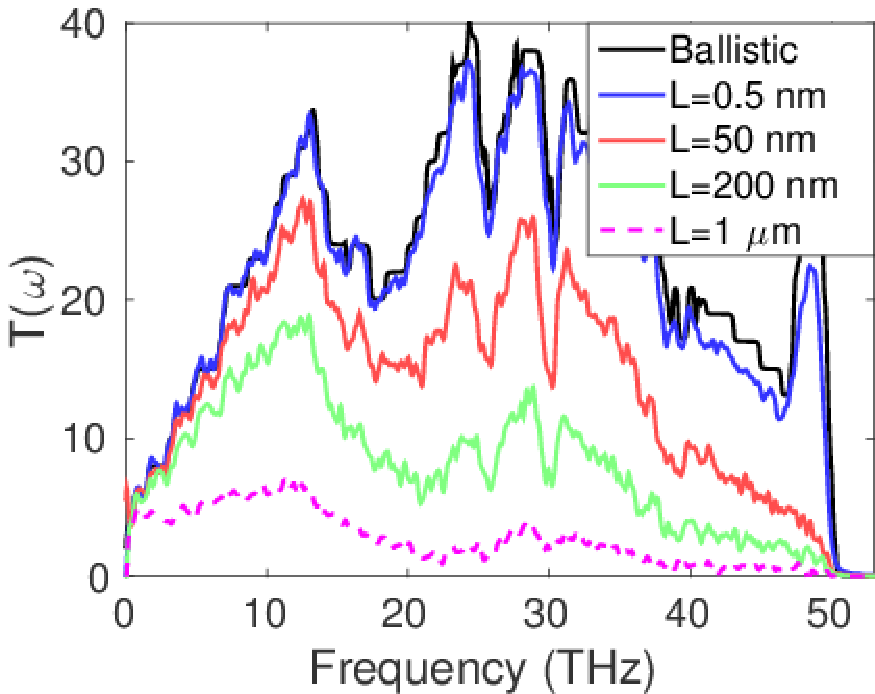
\includegraphics[width=.49\columnwidth]{pics/cnt_fig2.pdf} 
  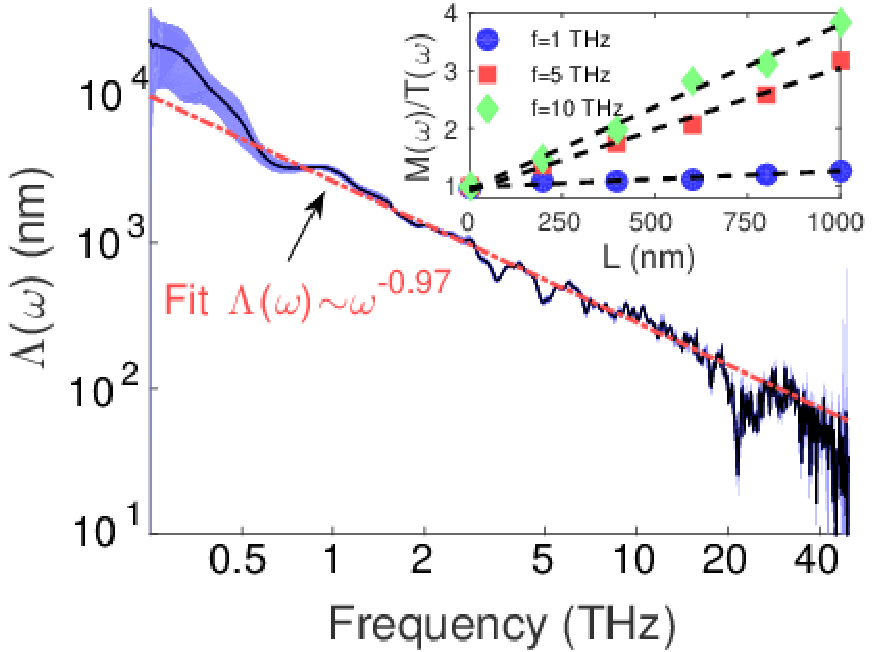
\includegraphics[width=.49\columnwidth]{pics/cnt_fig4.pdf} 
  \caption{(a) Generalized phonon transmission function $\ca{T}(\omega)=q(\omega)/(k_B\Delta T)$ for different tube lengths at $T=300$ K. Increasing the tube length reduces the transmission due to anharmonic scattering. For $L=0.5$ nm, phonon transmission is nearly equal to the ballistic value determined by counting the number of propagating modes in the nanotube. (b) Log-log plot of the mean free path $\Lambda(\omega)$ at $T=300$ K, determined from the slope of the inverse transmission function as a function of tube length $L$ as illustrated by the dashed lines in the inset. The shaded regions in the main figure correspond to the 92.5\% confidence interval for the slope. Below 0.25 THz, the confidence interval is large due to numerical uncertainties, preventing the determination of mean free paths at the lowest frequencies. Figure reprinted with publisher's permission from \citepub{cnt}. \textbf{ADD (A) AND (B)}}  
\label{fig:cnt_fig2}
 \end{center}
\end{figure}

Figure \ref{fig:cnt_fig2}(a) shows the generalized phonon transmission function $\ca{T}(\omega)=q(\omega)/(k_B\Delta T)$ for different tube lengths $L$. This dimensionless quantity essentially reflects the transmission probability through a tube of length $L$, summed over all propagating modes. For $L=0.5$ nm, the transmission probability of each mode is unity and the generalized phonon transmission is nearly equal to the number of propagating phonon modes (black solid line). As the tube length increases, anharmonic scattering reduces the transmission. This reduction is strongest at high frequencies, suggesting that the mean free path descreases as a function of frequency, which is in accordance with the larger phase-space available for phonon-phonon scattering at high frequencies \cite{ziman}.

Phonon mean free paths are plotted as a function of frequency in Fig. \ref{fig:cnt_fig2}. The mean free paths are calculated using the fitting procedure described in the inset of Fig. \ref{fig:cnt_fig2} and in more detail in \citepub{cnt}. The results show that the mean free paths obey a power-law $\Lambda(\omega)\propto \omega^{-\alpha}$ as a function of frequency in a large frequency interval, with a different exponent ($\alpha\approx 0.97$) than used earlier \cite{wang06_apl} to describe the ballistic-diffusive transition in CNTs ($\alpha=2$). At low frequencies, the MFPs exceed 1 $\mu$m, in accordance with the strong length-dependence of experimentally measured thermal conductivity in nanotubes as long as $5$ $\mu$m \cite{chang08}.

\subsection{Thermal conductivity reduction in twinning nanowires}

\label{sec:results_twinning}

\begin{figure}[tb]
 \begin{center}
  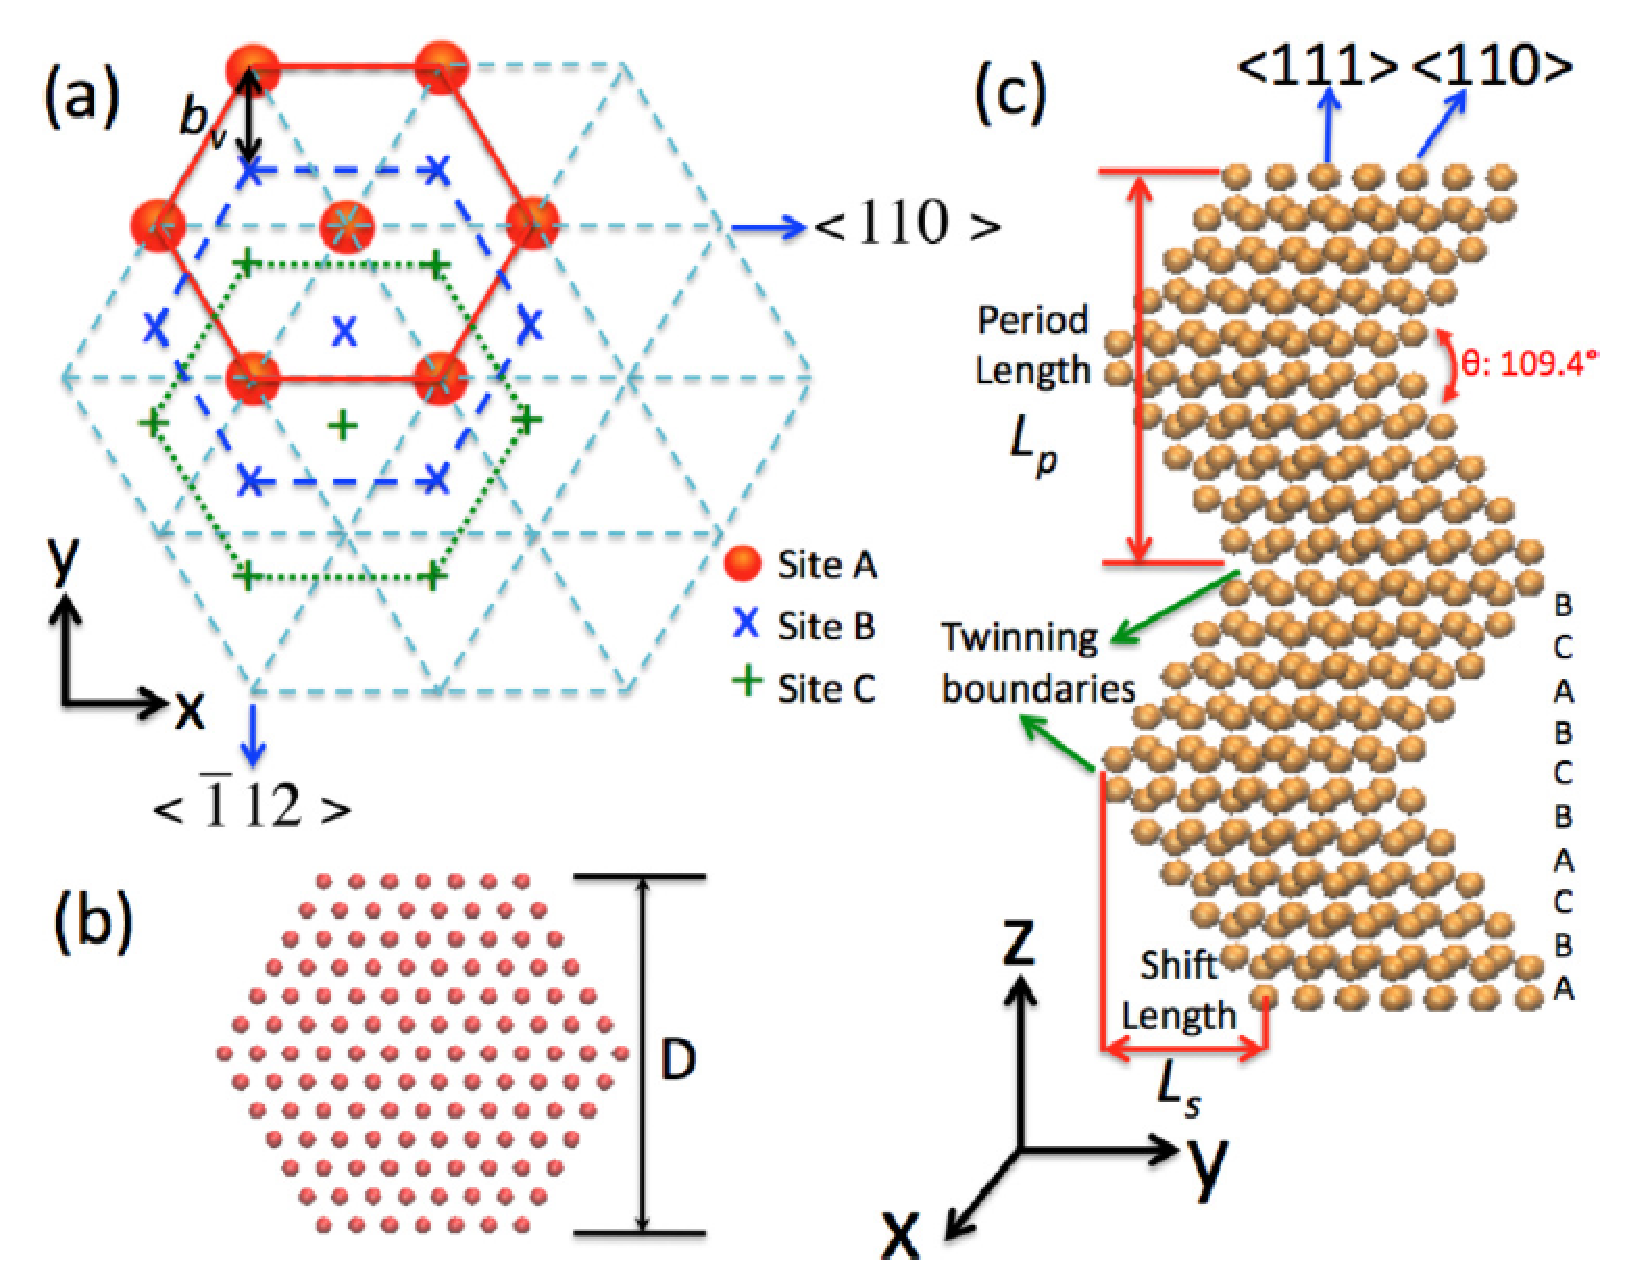
\includegraphics[width=.89\columnwidth]{pics/twinning_fig1.pdf} 
  \caption{(a) Schematic illustration of stacking in the close-packed silicon lattice. Stacking fault occurs when the stacking sequence ABCABC is locally changed to ABCBAC. (b) Cross-section of the nanowire. (c) Silicon nanowire with twinning boundaries. The period length is denoted by $L_p$ and the ''shift length'' $L_s$ is related to $L_p$ by $L_s=(L_p/2)\cot(\theta/2)$, where $\theta=109.4^{\circ}$. The figure also illustrates the perturbation of the ABCABC... stacking sequence at the twinning boundaries. Figure reprinted with publisher's permission from \citepub{twinning}.}  
\label{fig:twinning_fig1}
 \end{center}
\end{figure}

The geometry-induced effect of twinning on the thermal conductivity in silicon nanowires was investigated using NEMD in \citepub{twinning}. In twinning nanowires, phonons are scattered not only by anharmonic scattering as in the pristine nanotubes considered in the previous subsection but also by the twinning-induced zigzag-shaped kinks in the geometry. The possibility to tune the geometric parameters presents therefore opportunities for thermal conductivity engineering and, most crucially, reducing thermal conductivity without affecting electron transport. 

The computational NEMD setup of \citepub{twinning} was similar as for carbon nanotubes, with the small exception that Langevin heat baths were replaced by deterministic Nos\'e-Hoover thermostats \cite{nose84}. The cross-section of the nanowires was chosen to be hexagonal with diameter $D$ as shown in Fig. \ref{fig:twinning_fig1}(b). The twinning period is denoted by $L_p$, which corresponds to the ''shift length'' $L_s=(L_p/2)\cot(\theta/2)$, where $\theta=109.4^{\circ}$ [see Fig. \ref{fig:twinning_fig1}(c)]. Silicon-silicon interactions were modeled using the Stillinger-Weber many-body potential \cite{stillinger85}. More details are given in \citepub{twinning}.


\begin{figure}[tb]
 \begin{center}
  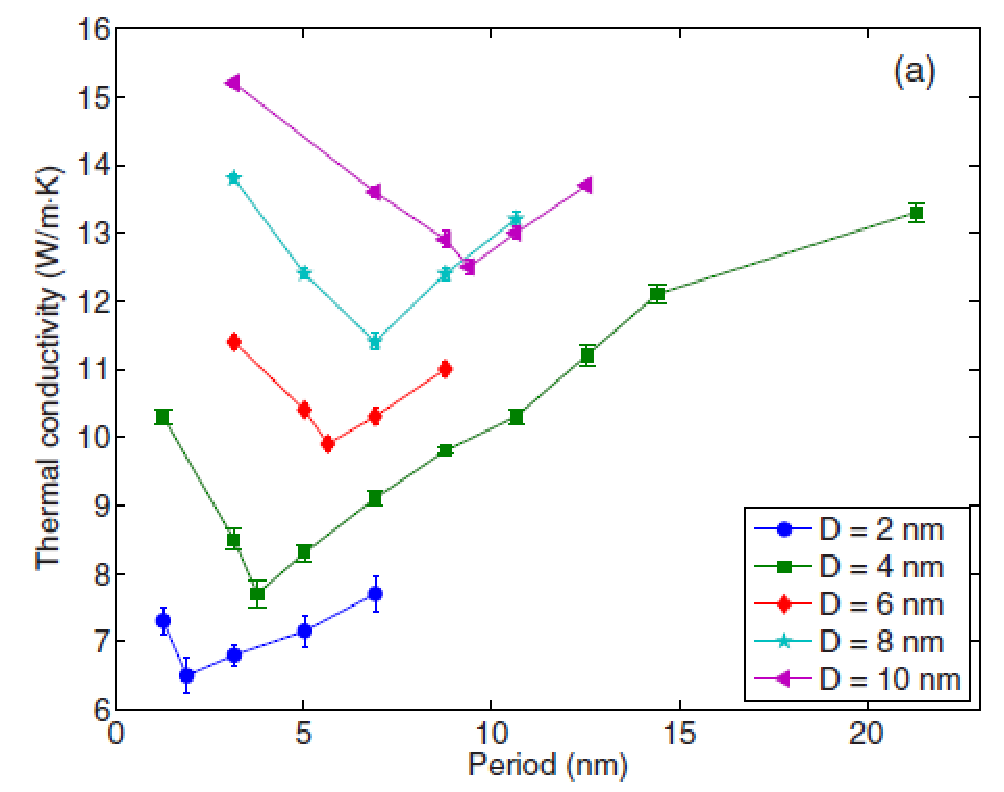
\includegraphics[width=.89\columnwidth]{pics/twinning_fig2a.pdf} 
  \caption{Thermal conductivity of silicon twinning nanowires at $T=300$ K as a function of period length $L_p$ for different diameters $D$. For each diameter $D$, there is a corresponding minimum in the thermal conductivity as a function of period length. The minimum arises from the competition between geometric and anharmonic effects as shown in \citepub{twinning}. Figure reprinted with publisher's permission from \citepub{twinning}. \textbf{REMOVE (A)}}  
\label{fig:twinning_fig2}
 \end{center}
\end{figure}

Thermal conductivity of the twinning nanowires as a function of period $L_p$ are shown in Fig. \ref{fig:twinning_fig2} for different diameters $D$. For each diameter, there is a corresponding period length with a minimum in the thermal conductivity. Phonon transport was found to be maximally hindered by the period length $L_p\approx 0.95D$, which corresponds to $L_s=D/3$. The detailed mechanisms underlying the minimum were analyzed in detail in \citepub{twinning}, with the conclusion that it arises from the competition between geometric and anharmonic scattering. To reduce TC even further, this geometric reduction can be used in conjuction with other well-known mechanisms for thermal conductivity reduction such as alloying \cite{}, partial amorphization \cite{}, and coating \cite{}. %  (see \citepub{twinning}). 

While the observed thermal conductivity minimum in twinning nanowires is analogous to the minimum thermal conductivity in superlattices (SLs) \cite{simkin00}, the mechanisms behind the phenomena are different. In SLs, the minimum arises from the interplay between phonon coherence and phonon boundary scattering, with the latter being due to acoustic mismatch at material interfaces. In twinning nanowires, there is no acoustic mismatch, so scattering only arises from the geometric effect. Because electron transport is expected to be unhindered by the stacking faults due to the small electron wavelength, the results suggest that the thermoelectric efficiency of twinning nanowires is higher than in their pristine counterparts. % This minimum was found to depend on the shift length as $L_s=D/3$, suggesting that the effect can be explained by geometric scattering. 


\section{Interference effects in phononic thermal conduction through constrictions (Publications \cp{fpu}, \cp{fpu2})}
\label{sec:results_interference}


\begin{figure}
\begin{center}
 %\includegraphics[width=8.6cm]{../scbaths_paper_re_resubmission/pic1.ps}
 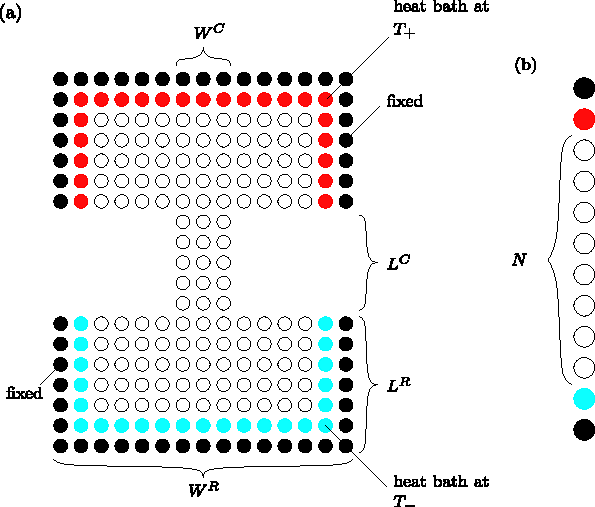
\includegraphics[width=.85\columnwidth]{pics/fpu_fig1.pdf}
 \caption{Schematic illustration of the simulation setup for a point contact in a two-dimensional square lattice. Figure reprinted with publisher's permission from \citepub{fpu}. \textbf{(b) TO BE REMOVED.}}
\label{fig:fpu_fig1}
\end{center}
\end{figure}

This section discusses interference effects in phononic thermal transport through nanoscale point contacts, studied in Publications \cp{fpu} and \cp{fpu2}. The NEMD simulation setup is schematically illustrated in Fig. \ref{fig:fpu_fig1}. Atoms are placed in a square lattice, with the particles at the boundaries of the bulk parts at the top or bottom being either fixed (black circles) or coupled to Langevin baths at temperature $T_+$ (red circles) or $T_-$ (cyan circles). In \citepub{fpu}, the large bulk parts were connected by a rectangular point contact that is $L^C$ atoms long and $W^C$ atoms wide. Triangular and discoidal shaped point contacts were considered in \citepub{fpu2}. 

Lattice dynamics is modeled by coupling nearest-neighbor atoms by anharmonic springs (not shown), whose potential energies include both quadratic and quartic terms. This potential was used by Fermi, Pasta and Ulam to investigate thermalization in one-dimensional systems \cite{fermi55} and is therefore called Fermi-Pasta-Ulam potential. The simple form of the Fermi-Pasta-Ulam potential allows for scaling the anharmonicity by a corresponding scaling in temperature, so one can present results for a single value of anharmonicity parameter without loss of generality. This scaling and other simulation details are presented in \citepub{fpu}. 


\begin{figure}
\begin{center}
 %\includegraphics[width=8.6cm]{../scbaths_paper_re_resubmission/pic1.ps}
 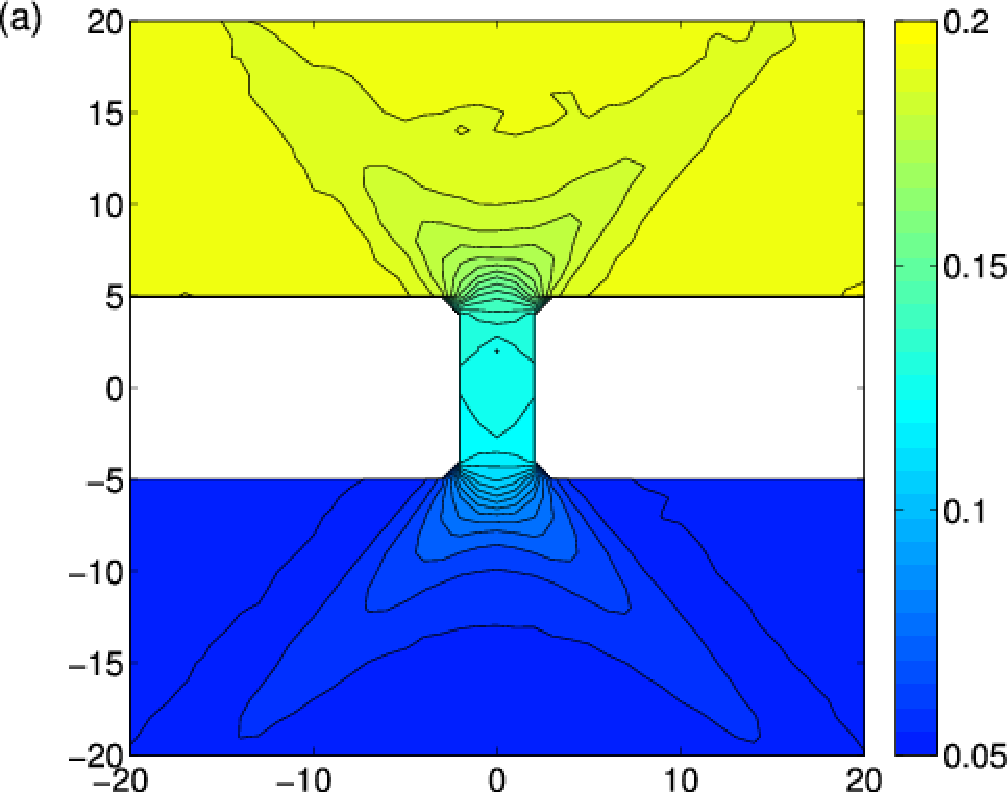
\includegraphics[width=.49\columnwidth]{pics/fpu_fig2a.pdf}
  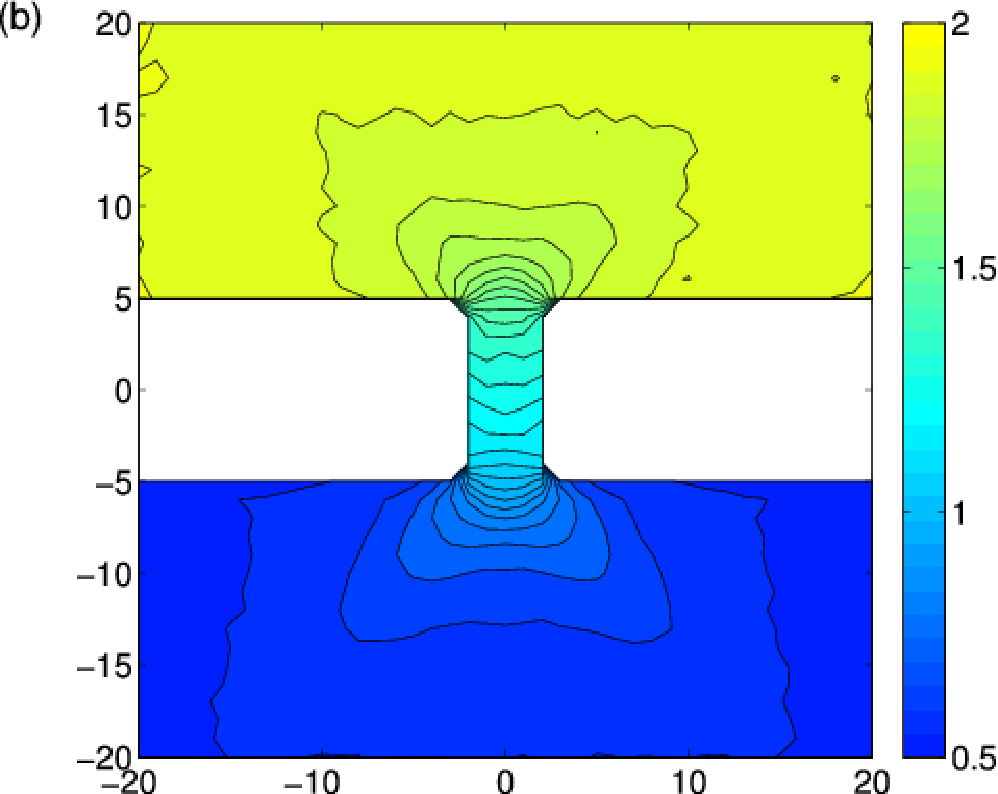
\includegraphics[width=.49\columnwidth]{pics/fpu_fig2b.pdf}
 \caption{Kinetic temperature profile at (a) low temperature ($T_+=0.20$, $T_-=0.05$) and (b) high temperature ($T_+=2.0$, $T_-=0.5$). The bulk size is $W^R=161$, $L^R=80$ and the constriction size $W^C=5$, $L^C=9$ (see Fig. \ref{fig:fpu_fig1}). The labels on the horizontal and vertical axes mark the atom indices. Figure reprinted with publisher's permission from \citepub{fpu}.}
\label{fig:fpu_fig2}
\end{center}
\end{figure}

Figure \ref{fig:fpu_fig2} shows the kinetic temperature $T_i^{\textrm{kin}}=\langle mv_i^2 \rangle/k_B$ at each atomic site $i$ in a contour plot at (a) low temperature and (b) high temperature for a rectangular constriction of length $L^C=9$ and width $W^C=5$. Temperatures are given in dimensionless units defined in \citepub{fpu}. At low temperature, lattice waves can propagate without losses and, therefore, temperature is nearly constant in the constriction. Most notably, the lossless propagation can be seen to induce wavelike-features in the kinetic temperature profile in the bulk parts,with directional features along the $\langle 11 \rangle$ crystal directions. Such features contrast with Fourier's law predicting a highly symmetric temperature profile with no directional features (not shown). When temperature is increased [Fig. \ref{fig:fpu_fig2}(b)], the directional features vanish and temperature profile becomes more similar to Fourier's law's prediction. Temperature profile also develops a non-zero gradient inside the constriction due to smaller thermal conductivity.


\begin{figure}
\begin{center}
 %\includegraphics[width=8.6cm]{../scbaths_paper_re_resubmission/pic1.ps}
 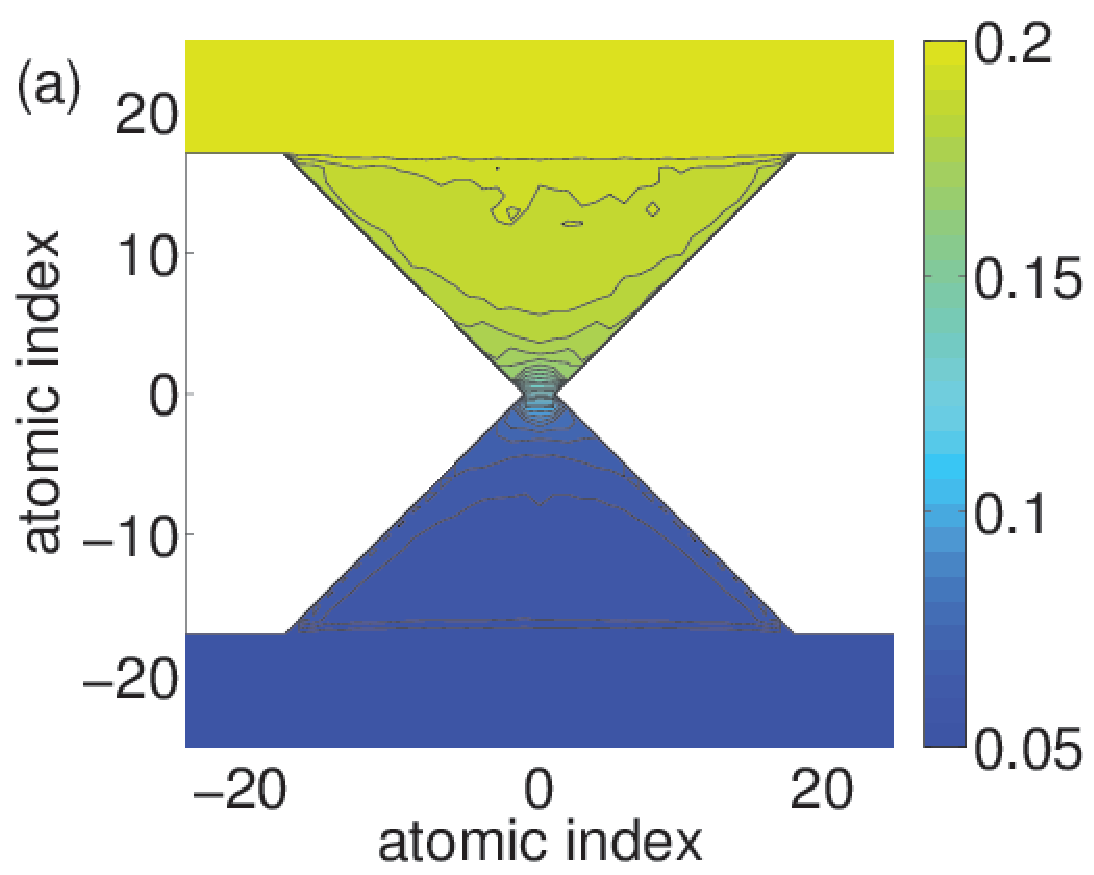
\includegraphics[width=.49\columnwidth]{pics/aip_fig5a.pdf}
 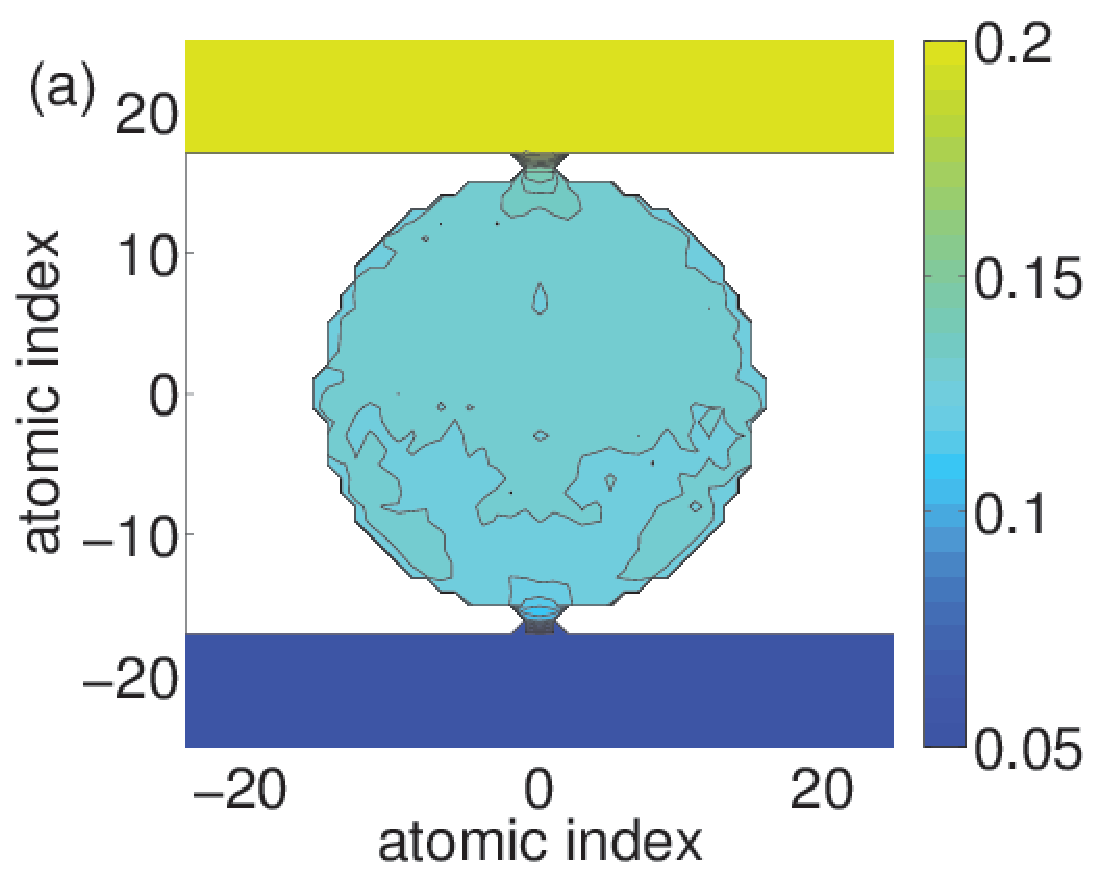
\includegraphics[width=.49\columnwidth]{pics/aip_fig6a.pdf}
 %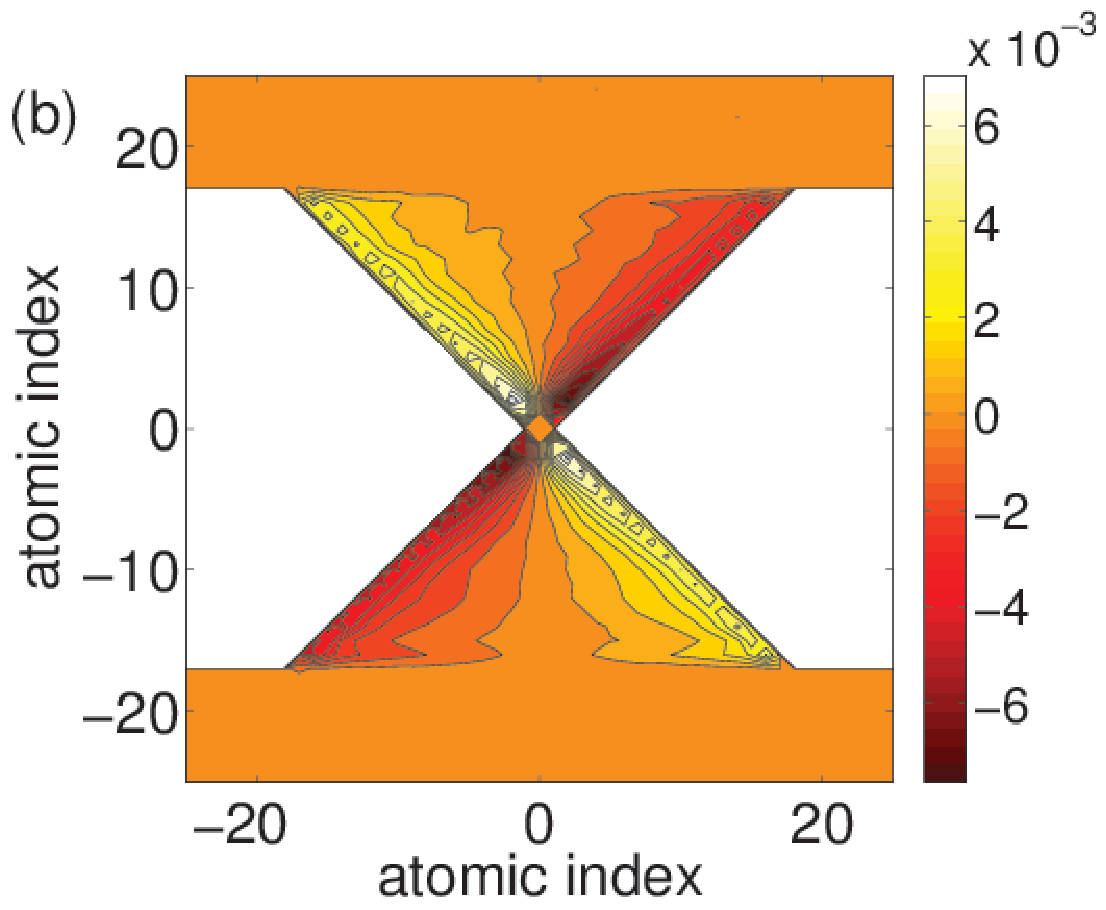
\includegraphics[width=.49\columnwidth]{pics/aip_fig5b.pdf}
 \caption{Kinetic temperature profile in (a) triangular and (b) discoidal constriction at low temperature. Figure reprinted with publisher's permission from \citepub{fpu2}. \textbf{FIX ANNOTATION IN B}}
\label{fig:aip_figs56}
\end{center}
\end{figure}

To investigate the effects of the constriction geometry on interference effects at low temperatures, calculations were performed also for hour-glass shaped and discoidal constrictions. Kinetic temperature profiles for these geometries are shown in Fig. \ref{fig:aip_figs56}. For the small contact areas shown here, temperature profiles in the bulk parts are essentially constant due to the small thermal contact between the upper and lower parts of the structure. In the triangular point contact, temperature changes nearly linearly as the constriction becomes narrower. Spatial analysis of the local heat current presented in \citepub{fpu2} reveals that heat flows mainly along the edges of the triangles. In the discoidal geometry of Fig. \ref{fig:aip_figs56}(b), which could represent a nanoparticle sandwiched between two materials, temperature profile is again nearly flat inside the center region, with only small spatial variations in temperature. However, local heat currents inside the center region, shown in \citepub{fpu2}, are strongly direction-dependent, with similar enhancement in $\langle 11\rangle$ direction as in the temperature profile of Fig. \ref{fig:fpu_fig2}(a).

The results show that in the ballistic low-temperature limit, local temperature and heat current profiles can exhibit wavelike-features with interference patterns. Accounting for such directional patterns could enable more efficient engineering of thermal conductivity in nanostructures. It is, however, well known that quantum statistics neglected by classical MD plays a significant role at low temperatures. To include quantum statistics, we turn to the quantum-mechanical Green's function method based on the linearized Langevin equations of motion presented in Sec. \ref{sec:th_eom}.

\section{Langevin models of lattice and electromagnetic energy transfer}
\label{sec:results_gf}

This section discusses quantum-mechanical energy transport by (i) phonons in point contacts (Subsection \ref{sec:results_schb}) and (ii) photons in mirror cavities (Subsection \ref{sec:results_cavity}). These analysis are based on solving the linearized Langevin equations of motion for phonons and photons, respectively, presented in Sec. \ref{sec:th_eom}. Quantum effects are incorporated through the quantum-mechanical fluctuation-dissipation theorem for Langevin noise terms (Sec. \ref{sec:th_langevin}) and dissipation effects through the Langevin damping terms accompanying the noise terms. % Losses are incorporated in the models through the Langevin terms. %Section \ref{sec:results_schb} presents quantum temperature profiles for rectangular point contacts ontacts and Section \ref{sec:results_cavity}  and (ii) electromagnetic energy transfer between nanoparticles in a mirror cavity. These results were published in Publications \cp{gf} and \cp{dipole}, respectively. 

\subsection{Quantum effects in constrictions (\citepub{gf}): Self-consistent heat bath model}
\label{sec:results_schb}

Application of the linearized Langevin equation \eqref{eq:th_eom1} for lossy phonon transport is known as the self-consistent heat bath model \cite{bolsterli70}. Whereas earlier works have applied the model to simple one-dimensional systems (see, e.g., Refs. \cite{bolsterli70,visscher75,dhar03,dhar06,segal09,bandyopadhyay11}) with a finite number of atoms, \citepub{gf} extended the model to more complex geometries with an infinite number of atoms.  %The model was then applied to investigating quantum temperature profiles in constrictions in rectangular lattices and graphene.

% An exemplary computational setup for vibrational heat transfer modeling is illustrated in Fig. \ref{fig:schb_setup} for a constriction in a two-dimensional lattice, studied in \citepub{gf}. Similar configuration was also applied to one-dimensional chains and a point contact in graphene in the same publication. 


The setup of \citepub{gf} is schematically illustrated in Fig. \ref{fig:schb_setup}. The setup consists of a center region with a finite number of atoms and left and right leads with possibly an infinite number of atoms. All atoms are coupled to local Langevin baths mimicking all interaction events driving the system towards local thermal equilibrium \cite{bolsterli70}. In the center region of Fig. \ref{fig:schb_setup}(a), a constriction acts as a scattering center for phonons coming in from the left and right leads. Around the constriction, bath temperatures are unknown, so they are determined self-consistently from the requirement that the heat current to each bath vanishes \cite{bolsterli70}. The requirement of zero heat current to local baths ensures that the heat current flowing in the chain is conserved at each atom site, a natural requirement in the steady-state. Away from the scattering region, the baths are set to prescribed temperatures $T_L$ and $T_R$. The modeling of atomic dynamics in the leads by Langevin terms contrasts with earlier works \cite{dhar06} and enables perfect acoustic matching between the leads and the center region, as discussed in \citepub{gf}.  % The baths then act as quantum-mechanical temperature probes. 


\begin{figure}
\begin{center}
 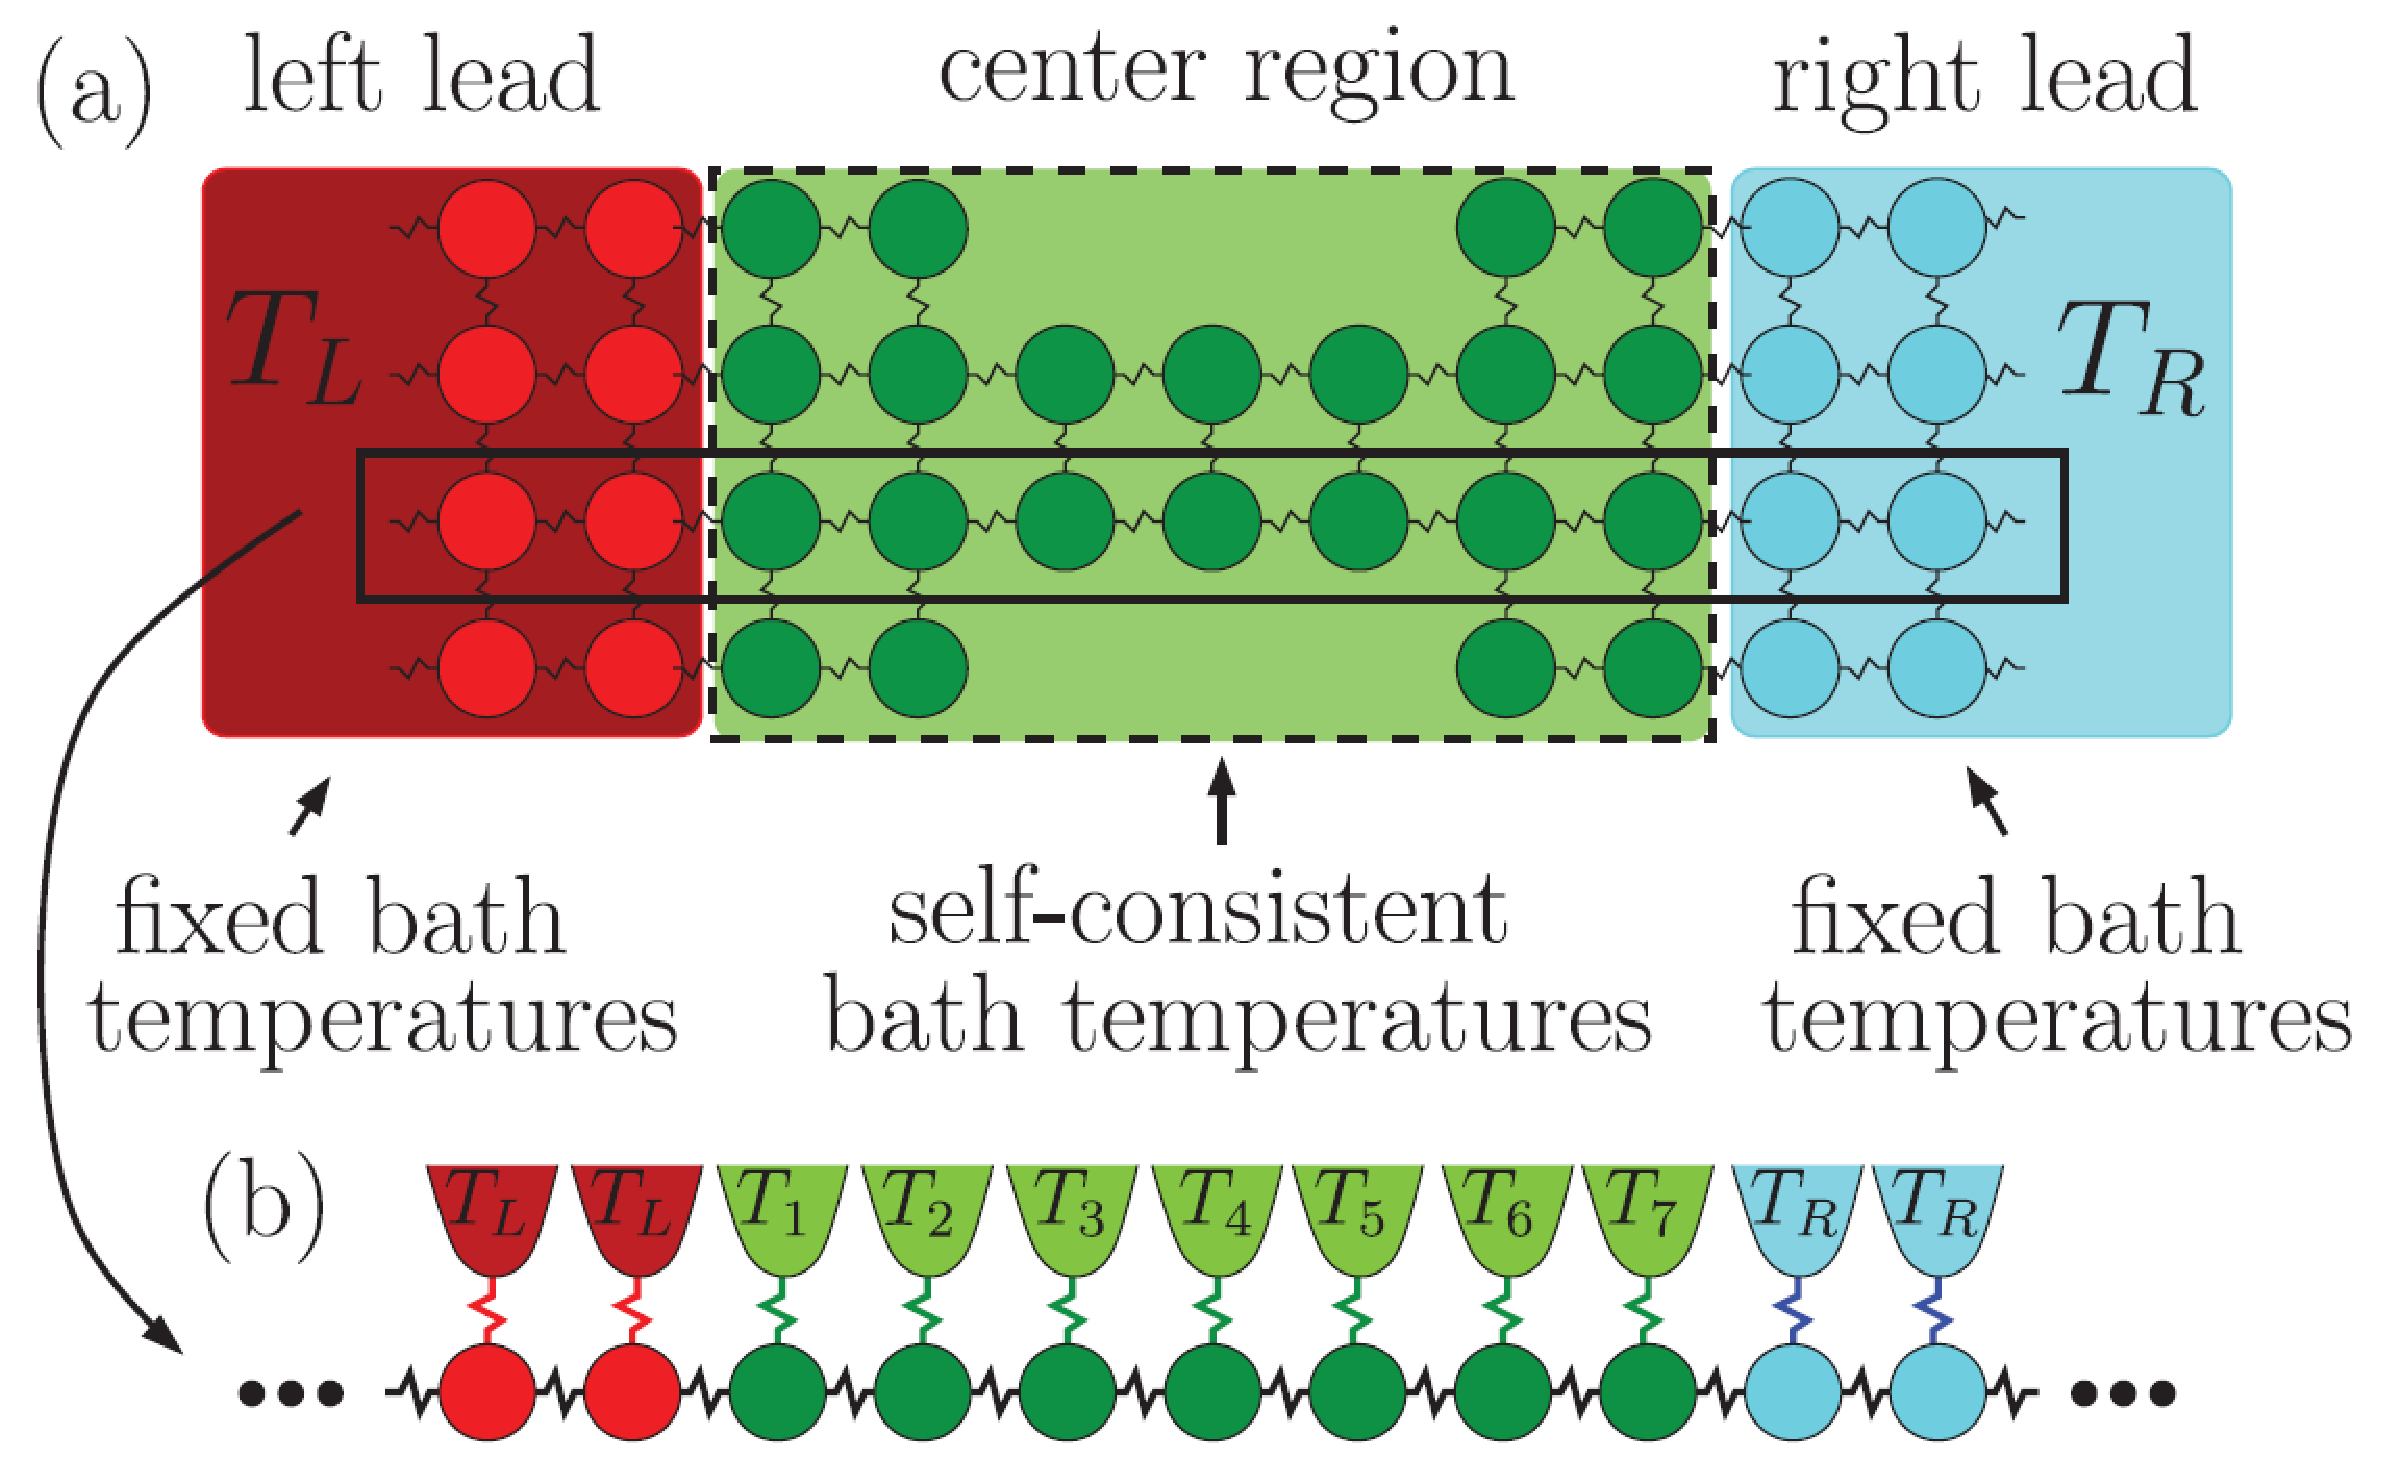
\includegraphics[width=.99\columnwidth]{pics/schb_setup.pdf}
 \caption{A schematic illustration of the self-consistent heat bath model for a constriction in a two-dimensional rectangular lattice. The system consists of the left lead, the center region, and the right lead. All atoms are coupled to Langevin heat baths, shown explicitly for one cross section in (b). Whereas the temperatures of the Langevin baths have prescribed values $T_L$ and $T_R$ in the left and right lead, the bath temperatures are determined self-consistently in the center region from the requirement that the thermal current to each bath is zero \cite{bolsterli70}. Reprinted from \citepub{gf} with publisher's permission.}
\label{fig:schb_setup}
\end{center}
\end{figure} 

% \begin{figure}
% \begin{center}
%  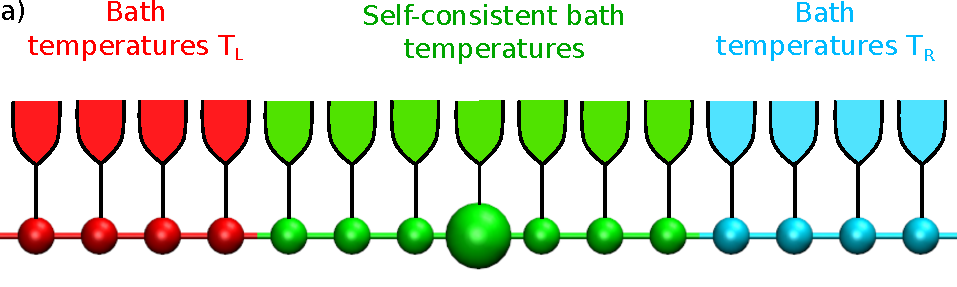
\includegraphics[width=.99\columnwidth]{pics/chain_rg.pdf}
%   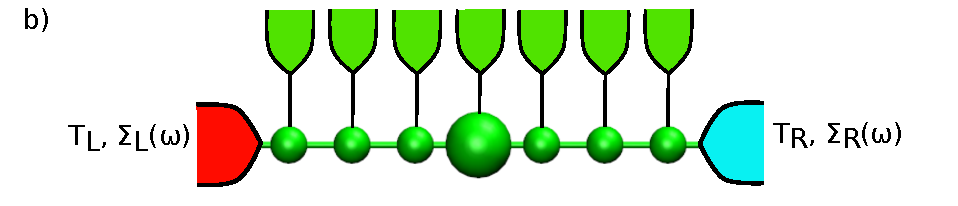
\includegraphics[width=.99\columnwidth]{pics/chain_rg2.pdf}
%  \caption{(a) Schematic illustration of the self-consistent bath model for an atomic chain with a mass defect. In the neighborhood of the mass defect acting as a scattering center, the bath temperatures are determined self-consistently from the requirement of vanishing heat current to the baths. In the left and right leads (red and blue, respectively), the bath temperatures are fixed at $T_L$ and $T_R$. (b) Illustration of the replacement of the leads by single Langevin heat baths at temperatures $T_L$ and $T_R$. The details of lattice dynamics in the leads is fully captured by the self-energy matrices $\Sigma^L(\omega)$ and $\Sigma^R(\omega)$, defined in detail in \citepub{gf}.}
% \label{fig:chain_rg}
% \end{center}
% \end{figure} 


The calculation of heat currents starts from writing down the Langevin equation of motion \eqref{eq:th_eom1} for each atom $i$ with interatomic force constants $\bb{K}_{ij}$ determined from interatomic potential energy as discussed in Sec. \ref{sec:th_eom2_phonon}. The relaxation rate $\gamma$ is chosen to correspond to known phonon life-times. It is shown in \citepub{gf} that solving the equations of motion for the leads and substituting to the equations for the center region allows for replacing the leads by \textit{single} Langevin heat baths at temperatures $T_L$ and $T_R$, which reduces the number of degrees of freedom to those in the center region. The microscopic details of lattice dynamics in the leads are fully captured by the lead self-energy functions $\Sigma^L(\omega)$ and $\Sigma^R(\omega)$. Microscopic definitions of the self-energy function in terms of the lead Green's function and the fluctuation-dissipation theorem for the corresponding Langevin noises are presented in detail in \citepub{gf}.



% The self-consistent bath model can be similarly extended for complex electron systems to study local heating and thermoelectric effects in quantum transport \cite{roy07}. 
% The heat current to each local bath at site $i$ can be determined by calculating the rate of change of local energy \cite{hardy63}, which reads in the harmonic approximation
% \begin{equation}
%  e_i = \frac{1}{2}m\dot{\bu}_i^2 + \frac{1}{2} \sum_{\alpha,\beta}\sum_j u_i^{\alpha} K_{ij}^{\alpha\beta} u_j^{\beta} . \label{eq:th_ei}
% \end{equation}
% Calculating the time derivative of Eq. \eqref{eq:th_ei} and thermal averaging gives
% \begin{equation}
%  \langle \dot{e}_i \rangle = -\sum_j  J_{ij} -  Q_i ,
% \end{equation}
% where the first term in brackets on the right hand side corresponds to the heat current
% \begin{equation}
%  J_{ij} = \frac{1}{2} \sum_{\alpha,\beta} \left\langle \dot{u}_i^{\alpha}K_{ij}^{\alpha\beta} u_j^{\beta} - u_i^{\alpha} K_{ij}^{\alpha\beta} \dot{u}_j^{\beta} \right\rangle
% \end{equation}
% between particles $i$ and $j$ and the second term is the heat flow to the bath, defined as 
% \begin{equation}
%  Q_i = \langle [m\gamma \dot{\bu}_i-\xi_i] \cdot \bu_i \rangle.
% \end{equation}


By following the procedure presented in Sec. \ref{sec:th_bathcurrents}, one can calculate the heat currents flowing to baths in terms of the center region's Green's function $\bb{G}(\omega)$. By setting the heat current equal to zero for the local baths in the center region, one gets a non-linear system of equations for the bath temperatures. This system of equations can be solved by, e.g., using Newton-Raphson method \cite{bandyopadhyay11} or resorting to linearizing approximations \cite{segal09}. The self-consistent temperature profile and the evaluation of heat currents flowing to the two leads then constitute a solution of the vibrational heat transfer problem. It is shown in \citepub{gf} that the requirement of vanishing heat current to the baths is equivalent to an intuitive thermal balance condition between kinetic and potential energies. Similar thermal balance condition was recently reported for local photon number in fluctuational electrodynamics \cite{partanen14}. %  temperature ensures local energy balance between the kinetic and potential energies. % Results for constrictions in two-dimensional lattices are presented in Sec. \ref{sec:results_gf}. %The transmission function is given by Eq. \eqref{eq:th_caroli} and $\Gamma^I(\omega)=-2\textrm{Im}[\Sigma^I(\omega)]$ is the bath coupling function, as again explained in \citepub{gf}.



% 

%The similarities of the equations of motion become more apparent in the linear approximation, which is discussed in more detail below. In this case, the force acting on atom $i$ becomes $F_i^{\alpha}=-\sum_{j}\sum_{\beta} K_{ij}^{\alpha\beta}u_j^{\beta}$ and the electron Hamiltonian 

% \subsubsection{Electromagnetic energy transfer in a cavity}

\begin{figure}
 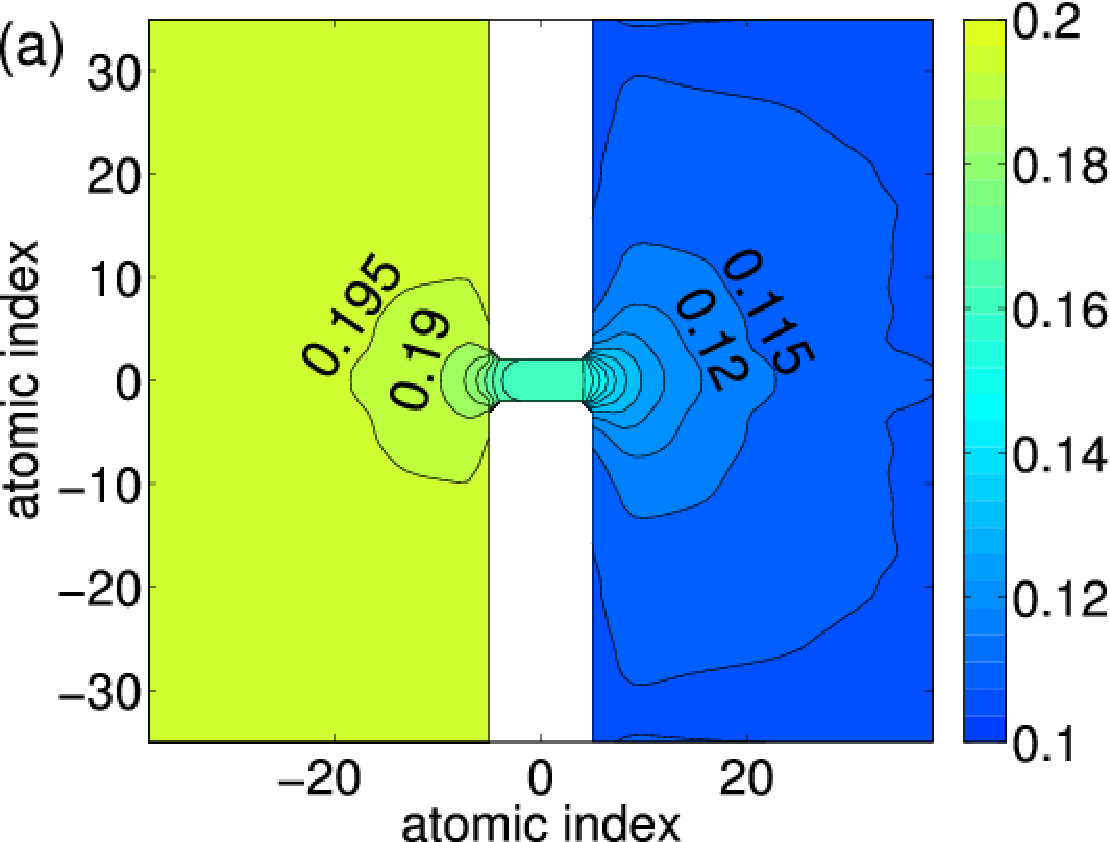
\includegraphics[width=.49\columnwidth]{pics/gf_fig7a.pdf}
 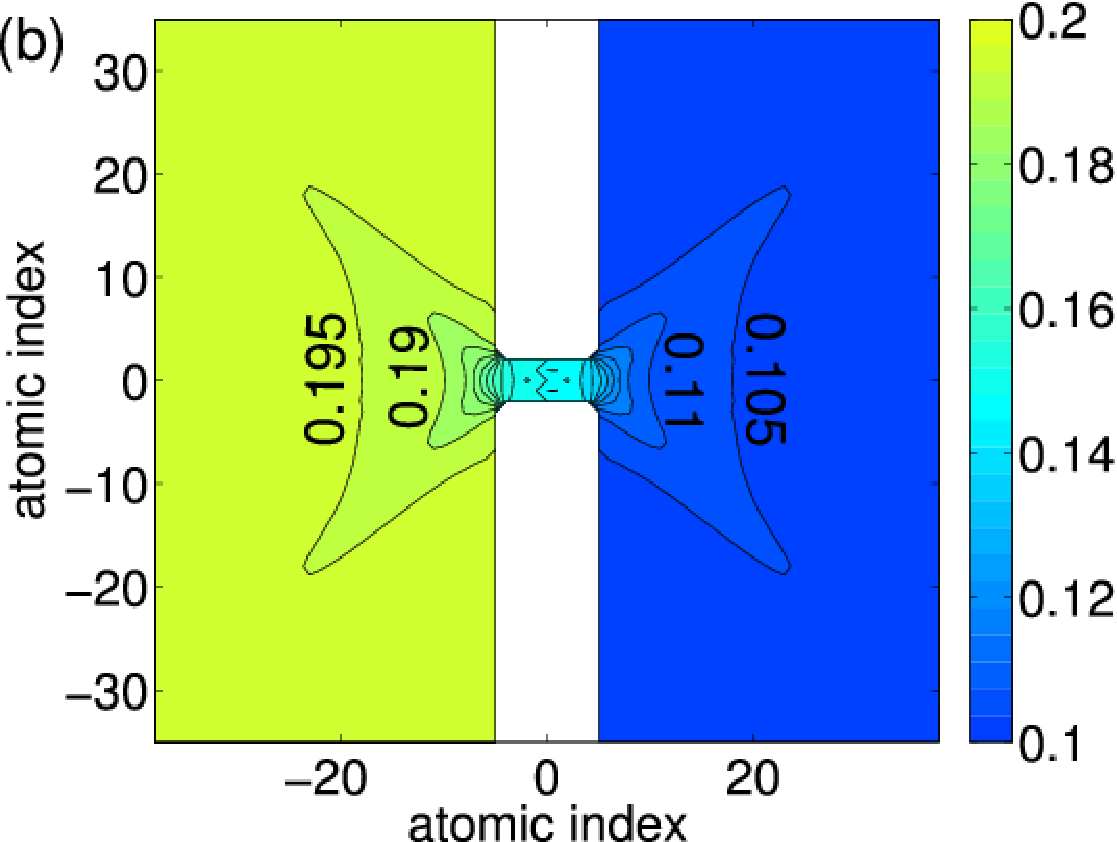
\includegraphics[width=.49\columnwidth]{pics/gf_fig7b.pdf}
 \caption{Self-consistent local bath temperature profiles in a rectangular constriction. Lead temperatures are $T_L=0.2$ and $T_R=0.1$. Figures show temperature profiles for (a) quantum and (b) classical statistics. Friction parameter is $\gamma=0.01$, corresponding to nearly ballistic transport. Figure reprinted with publisher's permission from \citepub{gf}.}
 \label{fig:gf_fig7}
\end{figure}

We first investigate quantum effects in the square lattice with a rectangular constriction. Nearest neighbors are connected by harmonic springs and weak dissipative losses are included through the bath dissipation parameter $\gamma=0.01$ (in the units of spring resonance frequency, see \citepub{gf}). Figure \ref{fig:gf_fig7} shows (a) quantum-statistical and (b) classical temperature profiles at low temperature. Results suggests that the directional features observed in the classical case may be washed away by quantum statistics, which modifies the mode occupation rates at high frequencies. 

\begin{figure}
 \begin{center}
 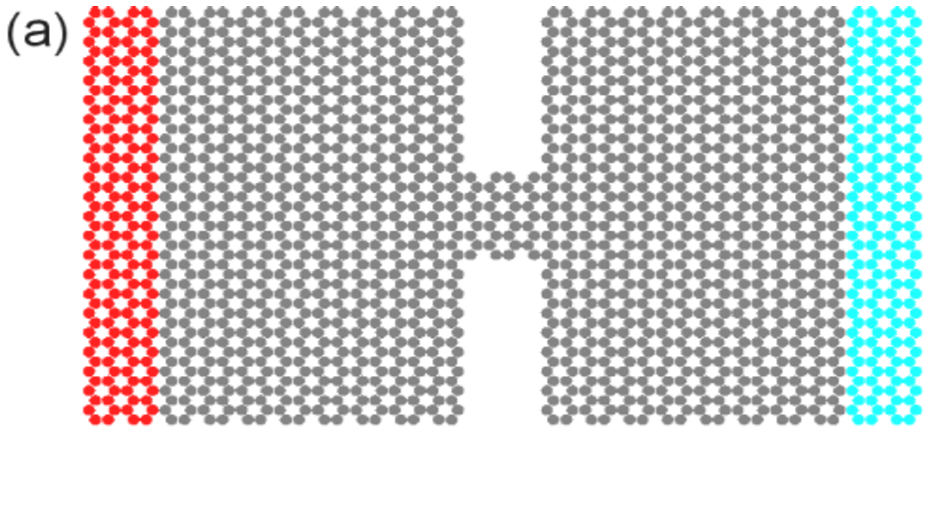
\includegraphics[width=.49\columnwidth]{pics/gf_fig8a.pdf}
 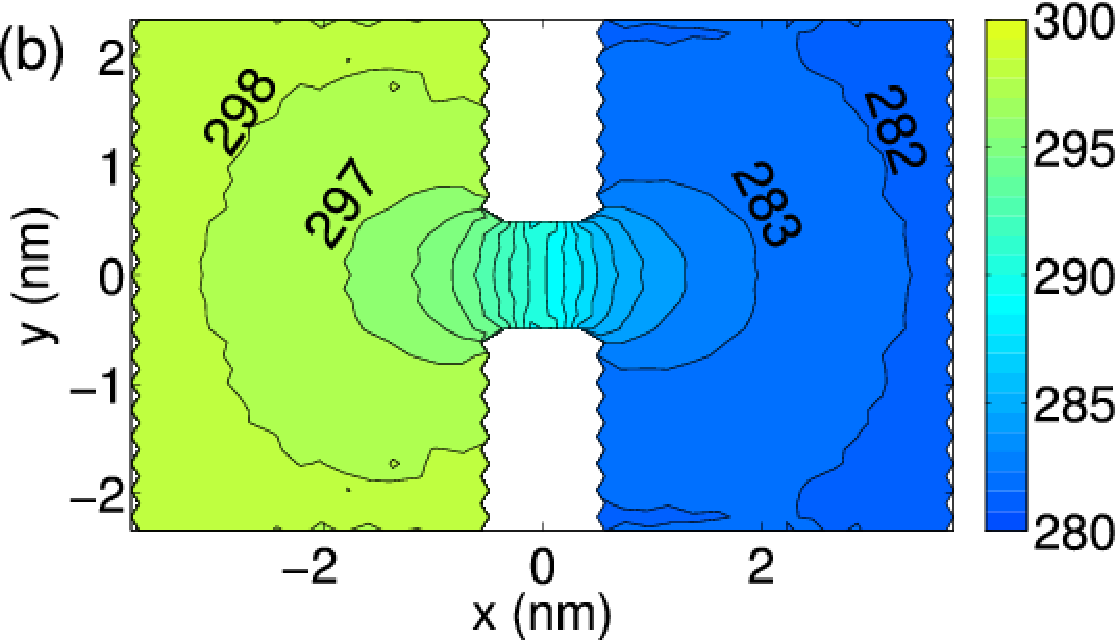
\includegraphics[width=.49\columnwidth]{pics/gf_fig8b.pdf}
 \end{center}
 \caption{(a) Graphene nanoconstriction. The leads extend infinitely to the left and right, but the temperatures are determined self-consistently only for the gray atoms in the shown center region. (b) Self-consistent bath temperature profiles (K). The semi-infinite leads are at temperatures $T_L=300$ K and $T_R=280$ K. The relaxation time $\tau=1/\gamma$ is set to $1$ ps. Figure reprinted with publisher's permission from \citepub{gf}.}
 \label{fig:gf_fig8}
\end{figure}

As a more realistic example, we consider quantum thermal transport through a constriction in graphene. Carbon-carbon interactions are modelled by...

The same principles as outlined here for phonon transport can be directly applied to electron transport as well, when the equations of motion are replaced by the electronic ones. In this case, the self-consistent baths are often referred to as voltage-temperature probes \cite{jacquet09}. Applications of voltage-temperature probe models for describing dissipation effects in electron transport have been so far limited only to one-dimensional geometries \cite{buttiker86,damato90,jacquet09,jacquet12}, although the model can account for wave dynamics, Joule heating as well as thermoelectric effects \cite{roy07}. Recently, Bergfield \textit{et al.} used the model for investigating quantum temperature oscillations in graphene \cite{bergfield15}.

\subsection{Cavity-modified electromagnetic energy transfer (\citepub{dipole})}
\label{sec:results_cavity}


